\documentclass{article}[11pt,subeqn]

\title{The Twin Instrument\footnote{We are grateful to Paul Devereux, 
James Fenske, Cheti Nicoletti, Atheen Venkataramani and Marcos Vera-Hernandez, 
along with seminar audiences and discussants at CMPO Bristol, ESPE, NEUDC, CSAE, 
The University of Essex, The University of Oxford and the Barcelona GSE summer 
forum for helpful comments.  We also are indebted to Emilia Del Bono, Climent 
Quintana-Domeque, Pedro R\'odenas, Anna Aevarsdottir, Martin Foureaux 
Koppensteiner and Ryan Palmer who have very kindly shared data and source code 
from their work.}}
\author{Sonia Bhalotra\thanks{The University of Essex.
Contact: srbhal@essex.ac.uk} 
\and Damian Clarke\thanks{The University of Oxford. 
Contact: damian.clarke@economics.ox.ac.uk}}
\date{\today}


%*******************************************************************************
\usepackage{amsmath}
\usepackage{amssymb}
\usepackage{appendix}
\usepackage{blindtext}
\usepackage{bm}
\usepackage{booktabs}
\usepackage{breqn}
\usepackage{caption}
\usepackage{color} \pagecolor{white}
\usepackage{dcolumn}
\usepackage{epsfig}
\usepackage{epstopdf}
\usepackage[capposition=top]{floatrow}
\usepackage{lastpage}
\usepackage{longtable}
\usepackage{lscape}
\usepackage{multirow}
\usepackage{natbib} \bibliographystyle{abbrvnat}\bibpunct{(}{)}{;}{a}{,}{,}
\usepackage{pdfpages}
\usepackage{rotating}
\usepackage{setspace}
\usepackage{subcaption}
\usepackage{url}
\usepackage{wrapfig}


%*******************************************************************************
\setlength\topmargin{-0.375in}
\setlength\textheight{8.8in}
\setlength\textwidth{5.8in}
\setlength\oddsidemargin{0.4in}
\setlength\evensidemargin{-0.5in}
\setlength\parindent{0.25in}
\setlength\parskip{0.25in}

\newcommand{\twinfolder}{"/home/damiancclarke/investigacion/Activa/Twins"}

%*******************************************************************************
\begin{document}
\begin{spacing}{1.4}

\maketitle
\begin{abstract}
 The incidence of twins has been used to identify the impact of changes in 
 fertility on measures of investment in children born prior to the twins, and
 the emerging consensus in this literature is that there is no evidence of a
 quantity-quality trade-off. We argue that the standard approach is flawed.
 Even if twin conception is random, bringing twins to term is a function of
 maternal health which is difficult to fully observe and which tends to be
 correlated with child quality, rendering the instrument invalid. The neglect
 of this fact in the existing literature will tend to lead to
 under-estimation of the quality-quantity (Q-Q) trade-off and so could
 contribute to explaining the negative results in the literature. Our contention
 that women who produce twin births are positively selected is demonstrated using
 data from richer and poorer countries. Using a large sample of microdata from
 developing countries which include indicators of maternal characteristics
 including health, we show that a significant trade-off emerges upon correcting
 for these biases. We show that this result is likely to be only a \emph{lower}
 bound of the true Q-Q trade-off and discuss how to estimate the size of these
 bounds.
 \\
\end{abstract}
\hspace{4mm}\textbf{\small JEL codes}: J12,J13,C13,D13,I12. \\

\newpage
%*******************************************************************************
\section{Introduction}                             \label{TWINscn:intro}
\section{The Twin Literature}                      \label{TWINscn:literature}
\section{Data and Estimation Samples}              \label{TWINscn:data}
\subsection{Data}                                  \label{TWINsscn:data}
\subsection{Estimation Samples}                    \label{TWINsscn:samples}
\subsection{Descriptive Statistics}                \label{TWINsscn:descriptives}
\section{Methodology}                              \label{TWINscn:method}
\subsection{Quantity-Quality with Twins}           \label{TWINsscn:methodQQ}
\subsection{Bounding the Q-Q Trade-off}            \label{TWINsscn:methodBounds}
\section{Results}                                  \label{TWINscn:results}
\section{Conclusion}                               \label{TWINscn:conclusion}

Section \ref{TWINscn:intro}
\newpage
\section*{Figures}
\begin{figure}[htpb!]
\centering
\begin{subfigure}{.5\textwidth}
  \centering
  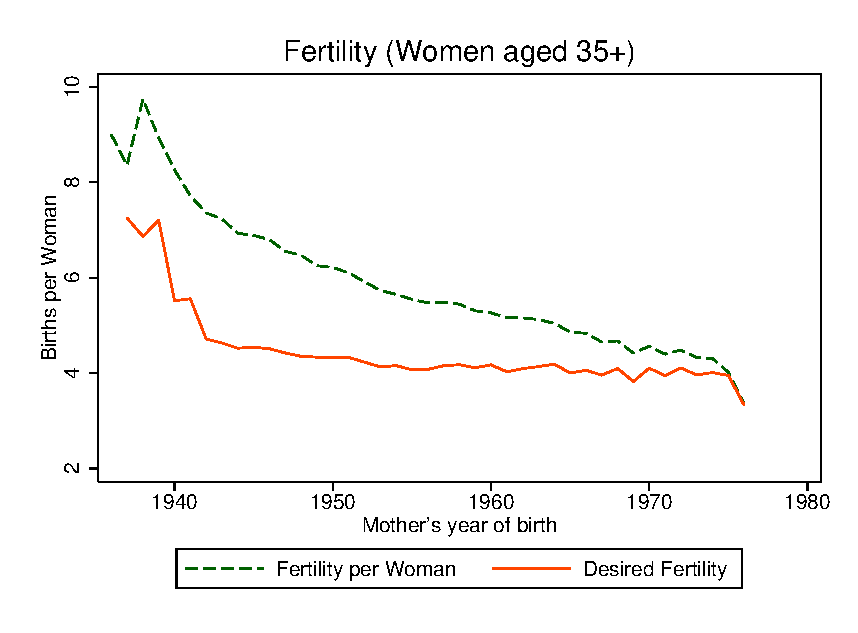
\includegraphics[scale=0.53]{\twinfolder/Figures/ferttrend_35_all.eps}
  \caption{Trends in Fertility}
  \label{TWINfig:fertrend}
\end{subfigure}%
\begin{subfigure}{.5\textwidth}
  \centering
  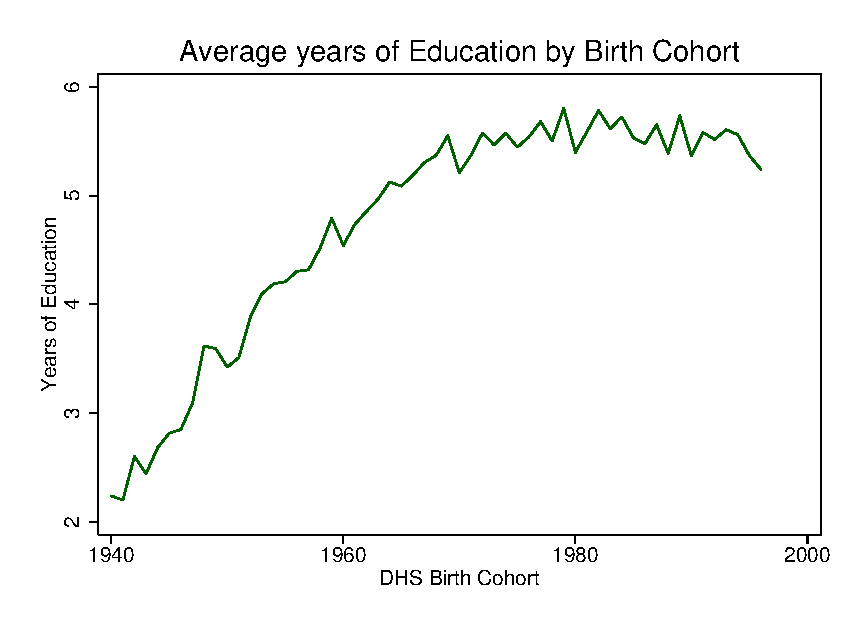
\includegraphics[scale=0.52]{\twinfolder/Figures/eductrend_all.eps}
  \caption{Trend in Education}
  \label{TWINfig:eductrend}
\end{subfigure}
\caption{Education and Fertility}
\label{TWINfig:trends}
\floatfoot{Note to figure \ref{TWINfig:trends}: Cohorts are made up of all individuals 
from the DHS who are over 35 years (for fertility), and over 15 years (for education).  
In each case the sample is restricted to those who have approximately completed fertility 
and education respectively.}
\end{figure}
\vspace{1cm}

\begin{figure}[htpb!]
\begin{center}
\caption{Proportion of Twins by Birth Order}
\label{TWINfig:bord}
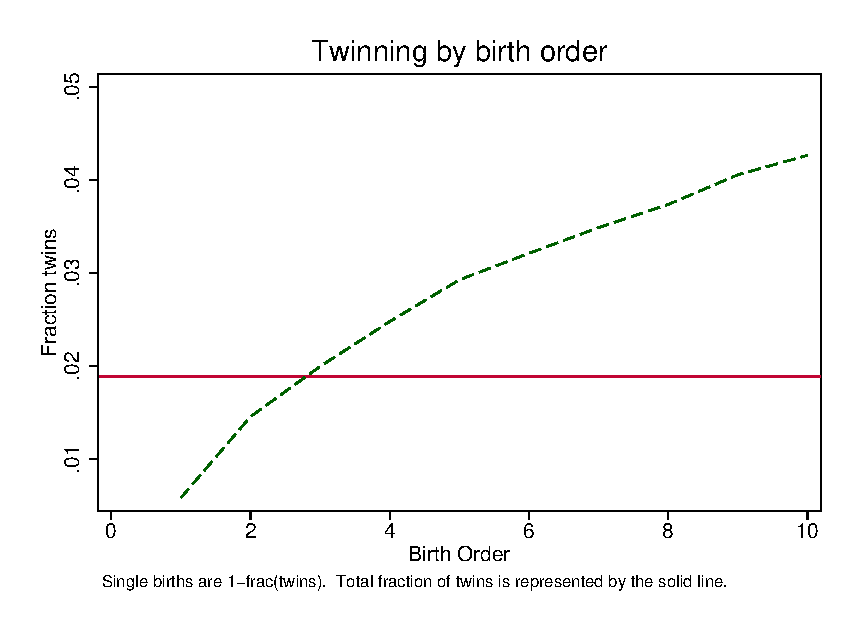
\includegraphics[scale=0.92]{\twinfolder/Figures/twinbybord.eps} 
\end{center}
\end{figure}

\begin{figure}[htpb!]
\begin{center}
\caption{Twin Births and Total Fertility}
\label{TWINfig:births}
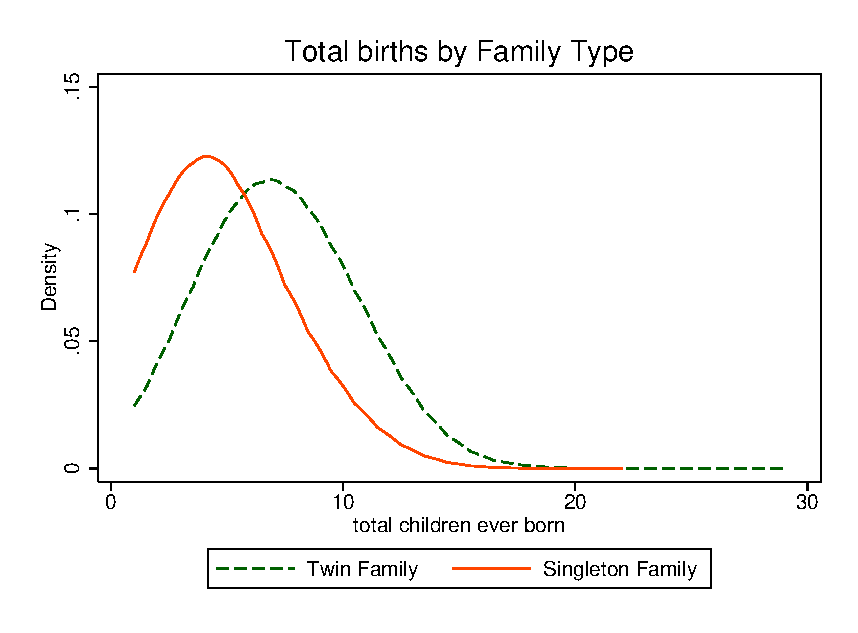
\includegraphics[scale=0.92]{\twinfolder/Figures/famsize.eps} 
\end{center}
\end{figure}

\begin{figure}[htpb!]
\begin{center}
\caption{Intra- and Inter-country trends: height and twinning}
\label{TWINfig:arrows}
\includegraphics[scale=0.86]{\twinfolder/Figures/height_country.eps} 
\end{center}
\end{figure}

\begin{figure}[htpb!]
\begin{center}
\caption{Proportion of Twins of All Births (USA)}
\label{TWINfig:USTwin}
\includegraphics[scale=0.92]{\twinfolder/Figures/USTwinFLE.eps} 
\end{center}
\end{figure}

\begin{figure}[htpb!]
\begin{center}
\caption{Relaxing Strict Exogeneity (two plus)}
\label{TWINfig:ltz2}
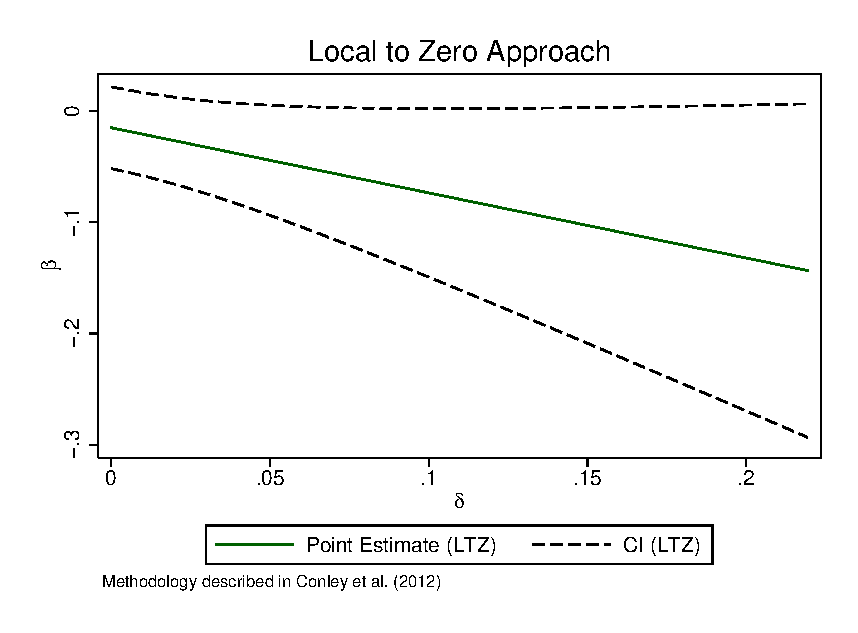
\includegraphics[scale=0.88]{\twinfolder/Figures/LTZ_two.eps}
\vspace{-8mm}
\floatfoot{Note to figure \ref{TWINfig:ltz2}: See note to Figure \ref{TWINfig:ltz3}}
\end{center}
\end{figure}

\begin{figure}[htpb!]
\begin{center}
\caption{Relaxing Strict Exogeneity (three plus)}
\label{TWINfig:ltz3}
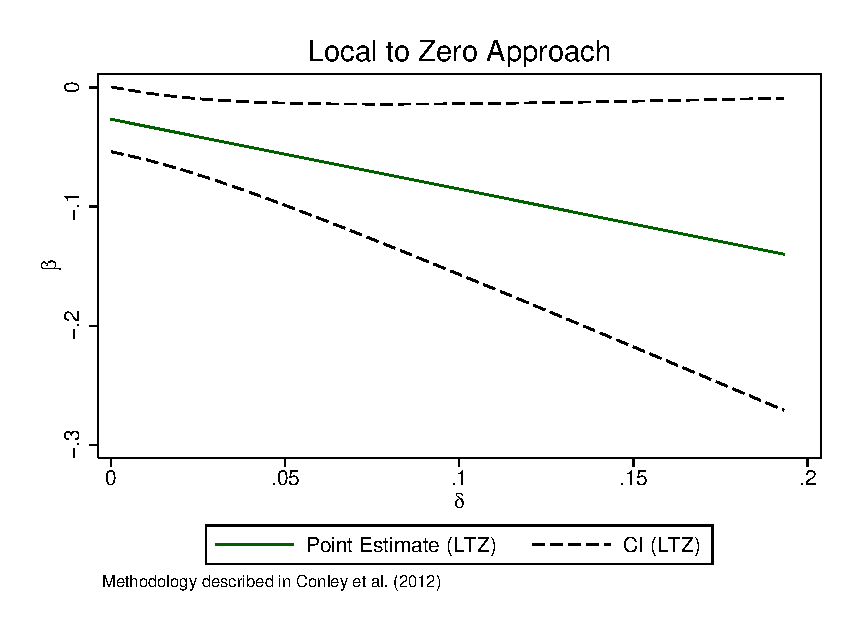
\includegraphics[scale=0.88]{\twinfolder/Figures/LTZ_three.eps} 
\floatfoot{Note to figure \ref{TWINfig:ltz3}: Confidence intervals and point estimates 
are calculated according to \citet{Conleyetal2012}.  Estimates reflect a range of priors 
regarding the validity of the exclusion restriction required to consistently estimate 
$\hat\beta_{fert}$ using twinning in a 2SLS framework.  The local to zero (LTZ) 
approach applied here assumes that $\gamma$, the sign on the instrument when included
in the first stage, is distributed $\gamma\sim U(0,\delta)$.  Further discussion 
is provided in the body of the text and table \ref{TWINtab:Conley}.}
\end{center}
\end{figure}




\clearpage
\section*{Tables}

\begin{landscape}\begin{table}[htpb!] 
\caption{Probability of Giving Birth to Twins} \label{TWINtab:twinreg1} 
\begin{center}\begin{tabular}{lcccccc} \toprule \toprule 
&(1)&(2)&(3)&(4)&(5)&(6)\\
Twin*100&All&\multicolumn{2}{c}{Income}&\multicolumn{2}{c}{Time}&Prenatal\\
 \cmidrule(r){3-4} \cmidrule(r){5-6} 
&&Low inc&Middle inc&1990-2013&1972-1989&\\\midrule
\begin{footnotesize}\end{footnotesize}&\begin{footnotesize}\end{footnotesize}&\begin{footnotesize}\end{footnotesize}&\begin{footnotesize}\end{footnotesize}&\begin{footnotesize}\end{footnotesize}&\begin{footnotesize}\end{footnotesize}&\begin{footnotesize}\end{footnotesize}\\
Age&0.596***&0.615***&0.554***&0.647***&0.326***&0.631***\\
&(0.029)&(0.036)&(0.050)&(0.033)&(0.075)&(0.040)\\
Age Squared&-0.008***&-0.008***&-0.008***&-0.009***&-0.003**&-0.009***\\
&(0.001)&(0.001)&(0.001)&(0.001)&(0.001)&(0.001)\\
Age First Birth&-0.053***&-0.093***&0.004&-0.052***&-0.056***&-0.041***\\
&(0.009)&(0.012)&(0.014)&(0.010)&(0.019)&(0.013)\\
Education (years)&0.042**&0.089***&-0.005&0.048**&0.022&-0.068**\\
&(0.017)&(0.022)&(0.029)&(0.020)&(0.034)&(0.028)\\
Education squared&-0.002&-0.006***&0.001&-0.002&0.000&0.003\\
&(0.001)&(0.002)&(0.002)&(0.002)&(0.003)&(0.002)\\
Height&0.058***&0.057***&0.059***&0.062***&0.042***&0.058***\\
&(0.004)&(0.005)&(0.007)&(0.005)&(0.008)&(0.007)\\
BMI&0.048***&0.063***&0.039***&0.046***&0.055***&0.044***\\
&(0.006)&(0.009)&(0.009)&(0.007)&(0.011)&(0.011)\\
Prenatal (Doctor)&&&&&&0.906***\\
&&&&&&(0.128)\\
Prenatal (Nurse)&&&&&&0.067\\
&&&&&&(0.108)\\
Prenatal (None)&&&&&&-0.497***\\
&&&&&&(0.132)\\
&&&&&&\\R-squared&0.01&0.01&0.01&0.01&0.01&0.01\\
Observations &1930653&1201555&729098&1524947&405706&615935\\
\hline\hline\multicolumn{7}{p{14.3cm}}{\begin{footnotesize}\textsc{Notes:} All specifications include a full set of year of birth and  country dummies, and are estimated as linear probability models.  Twin is multiplied by 100 for presentation.  Height is measured in cm  and BMI is weight in kg divided by height in metres squared. l  Prenatal care variables are only recoreded for recent births.  As  such, column (6) is estimated only for that subset of births where  these observations are made.
$^{*}$p$<$0.1; $^{**}$p$<$0.05; $^{***}$p$<$0.01
 \end{footnotesize}}\\ \hline \normalsize \end{tabular}\end{center}\end{table}\end{landscape} 

\begin{table}[htpb!]
\caption{United States Birth Registry (Administrative 2003-2012)}
\begin{center}
\scalebox{0.54}{
\begin{tabular}{lcccc} \hline
 & (1) & (2) & (3) & (4) \\
VARIABLES & twin100 & twin100 & twin100 & twin100 \\ \hline
\vspace{4pt} & \begin{footnotesize}\end{footnotesize} & \begin{footnotesize}\end{footnotesize} & \begin{footnotesize}\end{footnotesize} & \begin{footnotesize}\end{footnotesize} \\
africanAmerican & 0.554*** & 0.437*** & 0.437*** & 0.331*** \\
\vspace{4pt} & \begin{footnotesize}(0.00911)\end{footnotesize} & \begin{footnotesize}(0.0142)\end{footnotesize} & \begin{footnotesize}(0.0142)\end{footnotesize} & \begin{footnotesize}(0.0143)\end{footnotesize} \\
otherRace & 0.0433*** & 0.135*** & 0.135*** & -0.680*** \\
\vspace{4pt} & \begin{footnotesize}(0.00886)\end{footnotesize} & \begin{footnotesize}(0.0148)\end{footnotesize} & \begin{footnotesize}(0.0148)\end{footnotesize} & \begin{footnotesize}(0.0200)\end{footnotesize} \\
meducSecondary & 0.00124 & 0.0124 & 0.0124 & 0.810*** \\
\vspace{4pt} & \begin{footnotesize}(0.00881)\end{footnotesize} & \begin{footnotesize}(0.0159)\end{footnotesize} & \begin{footnotesize}(0.0159)\end{footnotesize} & \begin{footnotesize}(0.0203)\end{footnotesize} \\
meducTertiary & 1.124*** & 1.110*** & 1.110*** & 2.063*** \\
\vspace{4pt} & \begin{footnotesize}(0.00930)\end{footnotesize} & \begin{footnotesize}(0.0158)\end{footnotesize} & \begin{footnotesize}(0.0158)\end{footnotesize} & \begin{footnotesize}(0.0209)\end{footnotesize} \\
tobaccoUse & -0.327*** & -0.424*** & -0.424*** & -0.422*** \\
\vspace{4pt} & \begin{footnotesize}(0.0126)\end{footnotesize} & \begin{footnotesize}(0.0181)\end{footnotesize} & \begin{footnotesize}(0.0181)\end{footnotesize} & \begin{footnotesize}(0.0182)\end{footnotesize} \\
alcoholUse &  & -1.233*** & -1.233*** & -1.182*** \\
\vspace{4pt} & \begin{footnotesize}\end{footnotesize} & \begin{footnotesize}(0.0648)\end{footnotesize} & \begin{footnotesize}(0.0648)\end{footnotesize} & \begin{footnotesize}(0.0651)\end{footnotesize} \\
anemia &  &  &  & -1.349*** \\
\vspace{4pt} & \begin{footnotesize}\end{footnotesize} & \begin{footnotesize}\end{footnotesize} & \begin{footnotesize}\end{footnotesize} & \begin{footnotesize}(0.0335)\end{footnotesize} \\
diabetes &  &  &  & -0.408*** \\
\vspace{4pt} & \begin{footnotesize}\end{footnotesize} & \begin{footnotesize}\end{footnotesize} & \begin{footnotesize}\end{footnotesize} & \begin{footnotesize}(0.0280)\end{footnotesize} \\
chyper &  &  &  & -0.883*** \\
\vspace{4pt} & \begin{footnotesize}\end{footnotesize} & \begin{footnotesize}\end{footnotesize} & \begin{footnotesize}\end{footnotesize} & \begin{footnotesize}(0.0528)\end{footnotesize} \\
phyper &  &  &  & -4.128*** \\
\vspace{4pt} & \begin{footnotesize}\end{footnotesize} & \begin{footnotesize}\end{footnotesize} & \begin{footnotesize}\end{footnotesize} & \begin{footnotesize}(0.0267)\end{footnotesize} \\
eclamp &  &  &  & -5.686*** \\
\vspace{4pt} & \begin{footnotesize}\end{footnotesize} & \begin{footnotesize}\end{footnotesize} & \begin{footnotesize}\end{footnotesize} & \begin{footnotesize}(0.0896)\end{footnotesize} \\
Constant & 5.461*** & 5.326*** & 5.326*** & 32.75*** \\
 & \begin{footnotesize}(0.0525)\end{footnotesize} & \begin{footnotesize}(0.0806)\end{footnotesize} & \begin{footnotesize}(0.0806)\end{footnotesize} & \begin{footnotesize}(0.293)\end{footnotesize} \\
\vspace{4pt} & \begin{footnotesize}\end{footnotesize} & \begin{footnotesize}\end{footnotesize} & \begin{footnotesize}\end{footnotesize} & \begin{footnotesize}\end{footnotesize} \\
Observations & 38,910,055 & 16,605,619 & 16,605,619 & 12,219,256 \\
 $R^2$ & 0.008 & 0.008 & 0.008 & 0.012 \\ \hline
\multicolumn{5}{c}{\begin{footnotesize} Standard errors in parentheses\end{footnotesize}} \\
\multicolumn{5}{c}{\begin{footnotesize} *** p$<$0.01, ** p$<$0.05, * p$<$0.1\end{footnotesize}} \\
\end{tabular}}
\end{center}
\end{table}

\input{\twinfolder/Tables/TwinRegs/ChileTwin.tex}
\input{\twinfolder/Tables/TwinRegs/ScotlandTwin.tex}
\input{\twinfolder/Tables/TwinRegs/SwedenTwin2.tex}
\input{\twinfolder/Tables/Stress.tex}
\begin{table}[htpb]
\caption{Probability of Giving Births to Twins (NHIS, USA)}
\begin{center}
\scalebox{0.64}{
\begin{tabular}{lcc} \toprule
&(1)&(2) \\
VARIABLES&Twin$\times$100&Twin$\times$100 \\ \midrule
&& \\
Mother's Height&0.0416**&0.0406** \\
&(0.0201)&(0.0201) \\
Mother's Education&0.0084&0.0033 \\
&(0.0162)&(0.0164) \\
Smokes (pre-Pregnancy)&-0.119&-0.0983 \\
&(0.115)&(0.116) \\
Mother's Age&0.0121&0.0108 \\
&(0.0446)&(0.0446) \\
Mother's Age$^2$ &-0.0008&-0.0008 \\
&(0.0006)&(0.0006) \\
Age First Birth &0.166***&0.164*** \\
&(0.0135)&(0.0136) \\
BMI &0.0123***&0.0130*** \\
&(0.0034)&(0.0034) \\
Mother Good Health&&0.203* \\
&&(0.116) \\
Mother Poor Health&&-0.00284 \\
&&(0.189) \\
Constant&-4.091***&-4.101*** \\
&(1.542)&(1.543) \\
&& \\
Observations&105,879&105,879 \\
R-squared&0.004&0.004 \\ \midrule
%\multicolumn{3}{ p{5cm} }{\begin{footnotesize}\textsc{Notes:} Standard errors in parentheses. *** p$<$0.01; ** p$<$0.05; * p$<$0.1\end{footnotesize}}\bottomrule
\end{tabular}}
\end{center}
\end{table}

\input{\twinfolder/Tables/USfdeaths.tex}
\begin{table}
\caption{Twins, Miscarriage and Maternal Health (Administrative Data from Spain)}
\begin{center}
\scalebox{0.76}{
\begin{tabular}{lclc}
\hline 
VARIABLES	&	Fetal Death$	\times$100 & & \\	\hline
	&	(1) & &	\\
Primary	&	  -0.60179*** &	Primary$	\times$Twin	&	   -0.6618***	\\
	&	 (0.01456)	& &	 (0.20926)	\\
Secondary	&	  -0.71998*	& Secondary$	\times$Twin	&	  -0.55901***	\\
	&	  (0.0151)	& 	&	 .0020978	\\
Tertiary	&	  -0.80019***	& Tertiary$	\times$Twin	&	  -0.65091***	\\
	&	(0.01582)	& 	&	(0.20866)	\\
Immigration	&	  -0.07223***	& Immigration$	\times$Twin	&	  0.22871	\\
	&	 (0.0171)	& 	&	(0.29614)	\\
City	&	  -0.00321	& City$	\times$Twin	&	  0.09566	\\
	&	(0.01584)	& 	&	 (0.26876)	\\
Married	&	  -0.07354***	&Married$	\times$Twin	&	  -0.08978	\\
	&	 (0.00759)	&	&	 (0.11893)	\\
No Father	&	0.68626***	&No Father$	\times$Twin	&	3.25232	\\
	&	 (0.23825)	&	&	(4.09309)	\\
Constant	&	-1.35966***	& & \\
	&	(0.33674)	& &  \\
	& \\
	Obs & 2,869,329 & & \\
	$R^2$ & 0.0044  & & \\ \midrule
	\multicolumn{4}{p{8cm}}{Note: Spanish administrative births: 2007-2012.}
\end{tabular}}
\end{center}
\end{table}



\clearpage


\bibliography{./BiBBase1}

\newpage
\appendix
\section*{Appendices}
\section{Data Appendix}
\section{Appendix Tables}
\section{Appendix Figures}
\setcounter{figure}{0}
\renewcommand{\thefigure}{A\arabic{figure}}

\begin{figure}[htpb!]
\begin{center}
\caption{Birth Size of Twins versus Singeltons}
\label{TWINfig:Size}
\includegraphics[scale=0.90]{\twinfolder/Figures/Size.eps} 
\end{center}
\end{figure}

\begin{figure}[htpb!]
\begin{center}
\caption{Height and Selective Survival}
\label{TWINfig:survival}
\includegraphics[scale=0.90]{\twinfolder/Figures/MMRcuts.eps} 
\end{center}
\end{figure}

\begin{figure}[htpb!]
\begin{center}
\caption{Bootstrap Estimates of $\hat\gamma$}
\label{TWINfig:gammaBoots}
\includegraphics[scale=0.90]{\twinfolder/Figures/gammaResamp.eps} 
\end{center}
\floatfoot{Note to figure \ref{TWINfig:gammaBoots}: The empirical distribution
is generated by performing J=100 bootstrap replications to estimate $\phi_t$ and
$\phi_q$ (see discussion in appendix \ref{TWINscn:gamma}).  The analytical 
distribution is a normal $\sim N(\mu_{\hat\gamma},\sigma_{\hat\gamma})$.  The
values estimated in the bootstrap replications are $\mu_{\hat\gamma}=0.0642$ and
$\sigma_{\hat\gamma}=0.0493$.}
\end{figure}




\end{spacing}
\end{document}


%%********************************************************************************
Estimation of the Q-Q model using twin births to instrument fertility relies on 
the fact that twin births are exogenous. This implies that both conceiving twins 
\emph{and} taking them to term cannot depend on maternal behaviours and health 
stocks. In this paper we suggest that such an assumption may be too strong to 
hold in practice. We show that healthier mothers are more likely to give birth to 
twins even if twin conception is random, and that the size of this effect is 
considerable.

We re-estimate the Q-Q tradeoff accounting for such an effect.  We thus show
that the existing wisdom (which suggests that the effect of additional births 
on human capital might be minor), likely underestimates the true magnitude of
the Q-Q tradeoff.  Our IV estimates move point estimates from approximately 
0\% of a standard deviation (using the old methodology which does not account
for maternal health) to a significant $-4\%$ of a standard deviation of 
educational attainment.  Further, we suggest that this is likely
a lower bound of the true effect.  Depending upon the degree to which maternal
characteristics predict twin births, the true trade-off may be considerably
larger, perhaps even doubling these IV estimates.  The availability of richer 
maternal health and behaviour data in surveys would allow for us to restrict
the size of these bounds and produce more precise estimates.


